\documentclass[a4paper]{article}

\usepackage{lmodern}
\usepackage{graphicx}
\usepackage{subcaption}
\usepackage{parskip}
\usepackage{fullpage}


\title{INF4490 Mandatory assignment 1: \\
  Travelling Salesman Problem}
\author{Per Kulseth Dahl \\
{\tt pkdahl}}
\date{21 September 2018}

\begin{document}

\maketitle

\section*{Introduction}

This assignement was solved with Python 3.7. The only package used
that is not part of the Python Standard Library is matplotlib.
This package can be installed with pip, i.e. {\tt pip3 install matplotlib}.
I have used version 2.2.3 of the matplotlib package.

You may run the algorithms presented in this report with the same parameters and
on the same travelling salesman problem by running {\tt python3 main.py}.

\section*{Exhaustive search}

In the travelling salesman problem there are $n!$ different tours if we
have $n$ cities. Since it does not matter in which city we start a tour we
only need to check $(n-1)!$ of these tours. Additionally it does not matter
which direction we take a tour in so we can further divide the number of
tours we need to check in half. We therefore end up having to check
$(n-1)!/2$ tours in the exhaustive search.

\begin{table}[h]
  \centering
  \begin{tabular}{rrr@{ = }rr}
    Cities & Running & \multicolumn{2}{l}{Tours searched} & Tours searched \\
    & time & \multicolumn{2}{c}{} & per second \\
    \hline
    6 &   0.0003 & $5!/2$ & $60$ \\
    7 &   0.0020 & $6!/2$ & $360$ \\
    8 &   0.0127 & $7!/2$ & $2520$ \\
    9 &   0.1270 & $8!/2$ & $20160$ \\
    10 &  1.1503 & $9!/2$ & $181440$ & 157732 \\
    11 &  12.144 & $10!/2$ & $1814400$ & 149407 \\
    12 &  141.22 & $11!/2$ & $19958400$ & 141328 \\
  \end{tabular}
  \caption{Running time for exhaustive search with different number of cities.}
\end{table}

Assuming we can search 140000 tours per second and with 31557600 seconds
in a year it will take about 3~billion years to do an exhaustive search
for the best tour in our 24-city travelling salesman problem.

The shortest tour among the 10 first cities is of length 7486.

\newpage

\section*{Hill climbing}

In figure~\ref{fig:hc10} we see that our hill climber finds a tour very close
in length to the best tour almost every time. In our 20 runs only once it is
quite far off.

We see, as we would expect, that the standard deviation increases when we increase number of
cities in our travelling salesman problem.

The results of 20 runs of the hill climber on the first 10 cities and
all 24 cities are summarized in table~\ref{tab:hc}.

\begin{table}[h]
  \centering
  \begin{tabular}{lrr}
    & \multicolumn{2}{c}{Cities} \\
    & 10 & 24 \\
    \hline
    Best tour & 7486.3 & 12903.6 \\
    Worst tour & 8349.9 & 16101.5 \\
    Average tour & 7568.9 & 14429.6 \\
    Standard deviation & 205.2 & 709.0 \\
    Average running time & 0.098 & 0.578 \\
  \end{tabular}
  \caption{Statistics for the hill climber on
    the first 10 cities and all 24 cities over 20 runs.}
  \label{tab:hc}
\end{table}

\begin{figure}[h]
  \centering
  \begin{subfigure}[b]{0.48\textwidth}
    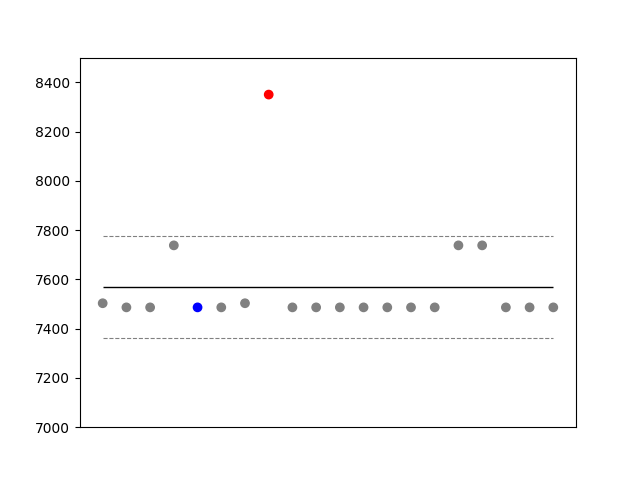
\includegraphics[width=\textwidth]{hill_climber_10.png}
    \caption{10 cities}\label{fig:hc10}
  \end{subfigure}
  \hfill
  \begin{subfigure}[b]{0.48\textwidth}
    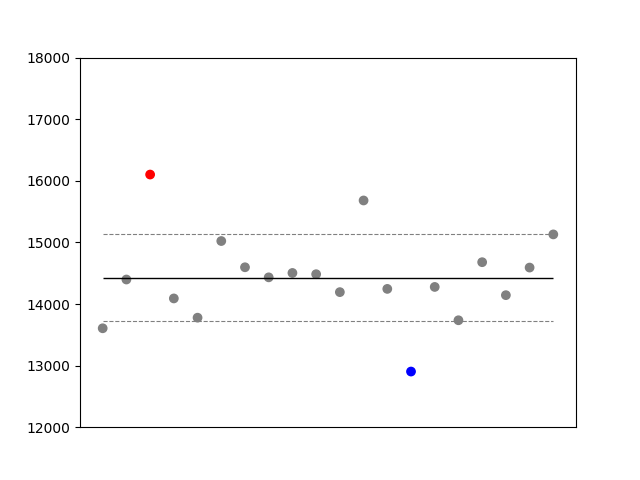
\includegraphics[width=\textwidth]{hill_climber_24.png}
    \caption{24 cities}\label{fig:hc24}
  \end{subfigure}
  \caption{Plots showing tour lengths found with the hill climber.}
\end{figure}

\newpage

\section*{Genetic algorithm}

The genetic algorithm first inititalizes with a randomly generated
population of tours. Then first an exploration phase is run before
an exploitation phase. The default is to run the first 60\%
generations in a exploration phase.

In the exploration phase stochastic universal sampling, partially
mapped crossover and scramble mutation is used for parent selection,
as crossover operator and as mutation operator, respectively.
Likewise, in the exploitation phase the operators as fitness proportional
sampling, edge recombination and swap mutation. In both phases replacement
is fitness based. The best 5\% or a minimum of the best 5 individual in a
population is kept from generation to generation.

\subsection*{10-city tours}

We see that the genetic algorithm finds the shortest tour in the
10-city travelling salesman problem on all 20 runs. The results are
summarized in table~\ref{tab:ga10} and figure~\ref{fig:ga10} shows
a plot. The algorithm was run with a population size of 200 and for
500 generations.

\begin{table}[h]
  \centering
  \begin{tabular}{lr}
    Best tour & 7486.31 \\
    Worst tour & 7486.31 \\
    Average tour & 7486.31 \\
    Standard deviation & 0.00 \\
    Average running time & 19.12 \\
  \end{tabular}
  \caption{Statistics for the genetic algorithm on
    the first 10 cities over 20 runs.}
  \label{tab:ga10}
\end{table}

\begin{figure}[h]
  \centering
  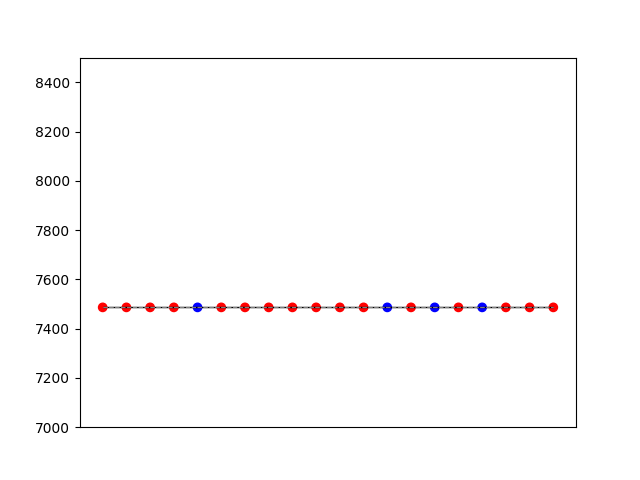
\includegraphics[width=0.48\textwidth]{genetic_10.png}
  \caption{Plot showing tour lengths found with the genetic algorithm
    on a 10-city travelling salesman problem.}
  \label{fig:ga10}
\end{figure}

\newpage

\subsection*{24-city tours}

The 24-city travelling salesman problem was run with population sizes of
50, 200 and 500 for 500 generations, and with population population sizes
of 25, 50 and 100 for 1000 generations. Each combinatoin was run 20 times.

The results are summarized in table~\ref{tab:ga24}. It seeems we get better
results running smaller populations for more generations than larger
populations for fewer generations.

\begin{table}[h]
  \centering
  \begin{tabular}{rrrrrrr}
    Population & Best & Worst & Average &
    Standard & Average & Generations \\
    size & tour & tour & tour & deviation & running & \\
    & & & & & time & \\
    \hline
    50 & 13368.5 & 17470.1 & 15470.3 & 1000.0 & 10.1 & 500 \\
    200 & 13493.3 & 16214.6 & 14756.9 & 829.2 & 41.9 & 500 \\
    500 & 12684.6 & 15187.1 & 14004.8 & 682.3 & 109.3 & 500 \\
    25 & 13057.1 & 15547.4 & 14317.0 & 824.0 & 10.2 & 1000 \\
    50 & 12842.6 & 16870.0 & 14013.8 & 1005.4 & 20.8 & 1000 \\
    100 & 12737.8 & 16630.8 & 14454.7 & 1039.1 & 39.6 & 1000 \\
  \end{tabular}
  \caption{Statisics for the genetic algorithm on
    all 24 cities over 20 runs.}
  \label{tab:ga24}
\end{table}

\begin{figure}[h]
  \centering
  \begin{subfigure}[b]{0.48\textwidth}
    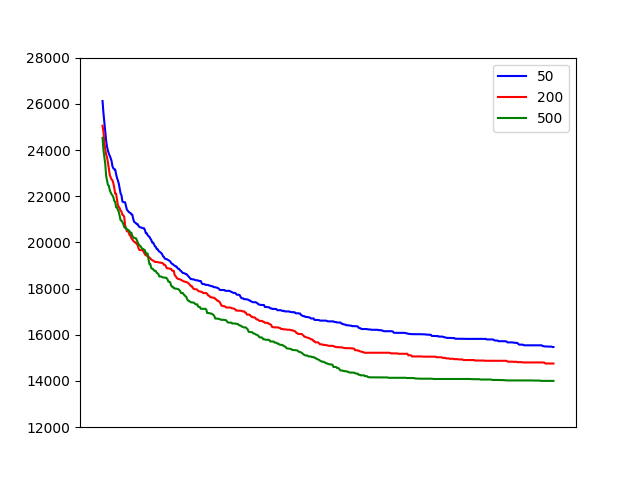
\includegraphics[width=\textwidth]{run_genetic_24_20_runs_500_gens.png}
    \caption{500 generations}
  \end{subfigure}
  \hfill
  \begin{subfigure}[b]{0.48\textwidth}
    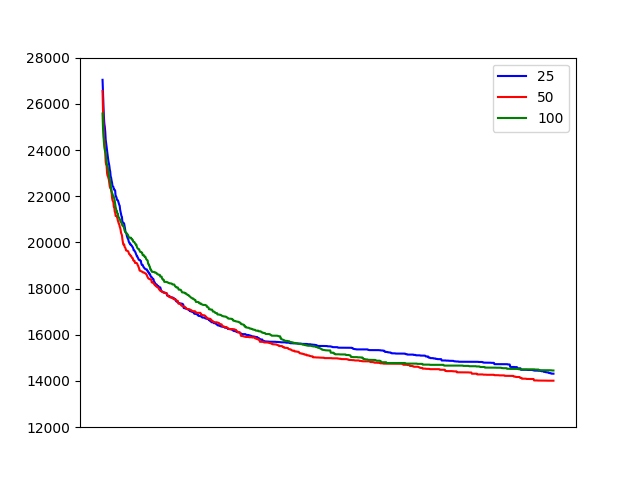
\includegraphics[width=\textwidth]{run_genetic_24_20_runs_1000_gens.png}
    \caption{1000 generations}
  \end{subfigure}
  \caption{Plot showing the average best tour in each generation
    over 20 runs with the genetic algorithm.}
\end{figure}

\newpage

\section*{Hybrid algorithm}

In the hybrid algorithm the selection of parents for the first generation
of offspring is a fintess proportional selection based on the fitness value
obtained from running the hill climber on the initial random population.
In the Lamarckian version the parent is replaced with the hill-climbed version
while in the Baldwinian the original parent is kept. After this inital the
algorithm is the same as the genetic.

\subsection*{Baldwinian}

We see that the Baldwinian version of the hybrid algorithm yields a result
very similar to that of the genetic algorithm.

The results are summarized in table~\ref{tab:hb} and plots showing the average
best in each generation is shown in figure~\ref{fig:hb}.

\begin{table}[h]
  \centering
  \begin{tabular}{rrrrrrr}
    Population & Best & Worst & Average &
    Standard & Average & Generations \\
    size & tour & tour & tour & deviation & running & \\
    & & & & & time & \\
    \hline
    50 & 13271.7 & 16463.1 & 15136.0 & 864.6 & 13.1 & 500 \\
    200 & 13079.3 & 16766.9 & 14411.7 & 967.1 & 52.9 & 500 \\
    500 & 12879.5 & 15845.6 & 13946.1 & 870.0 & 134.2 & 500 \\
    25 & 12807.4 & 15889.7 & 14260.2 & 939.2 & 11.0 & 1000 \\
    50 & 12423.0 & 15772.1 & 13764.1 & 887.9 & 22.0 & 1000 \\
    100 & 13078.0 & 15622.4 & 14467.6 & 776.4 & 47.0 & 1000 \\
  \end{tabular}
  \caption{Statistics for the Baldwinian version of the hybrid algorithm
    over 20 runs.}
  \label{tab:hb}
\end{table}

\begin{figure}[h]
  \centering
  \begin{subfigure}[b]{0.48\textwidth}
    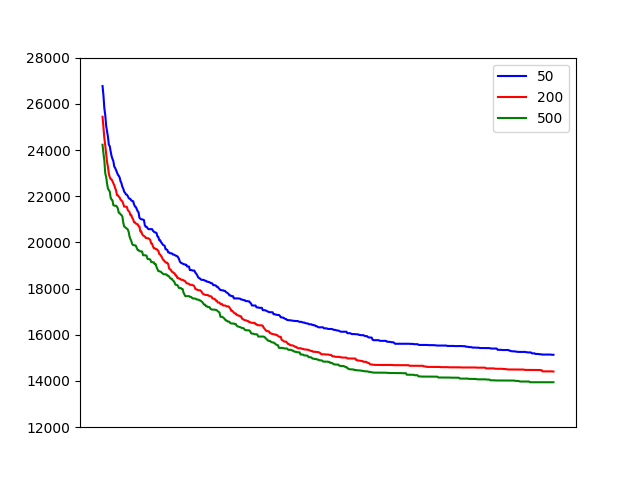
\includegraphics[width=\textwidth]{run_hybrid_baldwinian_20_runs_500_gens.png}
    \caption{500 generations}
  \end{subfigure}
  \hfill
  \begin{subfigure}[b]{0.48\textwidth}
    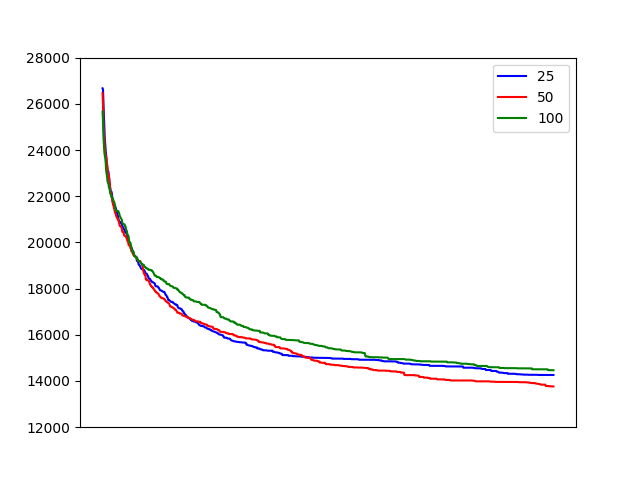
\includegraphics[width=\textwidth]{run_hybrid_baldwinian_20_runs_1000_gens.png}
    \caption{1000 generations}
  \end{subfigure}
  \caption{Plots showing the average best tour in each generation over 20 runs
    with the Baldwinian version of the hybrid algorithm.}
  \label{fig:hb}
\end{figure}

\newpage

\subsection*{Lamarckian}

With the Lamarckin version of the hybrid algorithm we start out with
solutions with close to local minima. Then in subsequent generations
there is little improvement. Because there is little room for improvement.
This can been seen very clearly in the plots shown in figure~\ref{fig:hl}.

The results are summarized in table~\ref{tab:hl}.

\begin{table}[h]
  \centering
  \begin{tabular}{rrrrrrr}
    Population & Best & Worst & Average &
    Standard & Average & Generations \\
    size & tour & tour & tour & deviation & running & \\
    & & & & & time & \\
    \hline
    50 & 12334.4 & 13753.0 & 12903.0 & 397.4 & 12.1  & 500 \\
    200 & 13057.1 & 15547.4 & 14317.0 & 824.0 & 10.2 & 500 \\
    500 & 12842.6 & 16870.0 & 14013.8 & 1005.4 & 20.8 & 500 \\
    25 & 12334.3 & 13977.6 & 12926.5 & 451.8 & 10.8 & 1000 \\
    50 & 12325.9 & 13351.0 & 12818.3 & 348.2 & 23.5 & 1000 \\
    100 & 12287.1 & 13424.0 & 12756.5 & 259.5 & 45.3 & 1000 \\
  \end{tabular}
  \caption{Statistics for the Lamarckian version of the hybrid algorithms
    over 20 runs.}
  \label{tab:hl}
\end{table}

\begin{figure}[h]
  \centering
  \begin{subfigure}[b]{0.48\textwidth}
    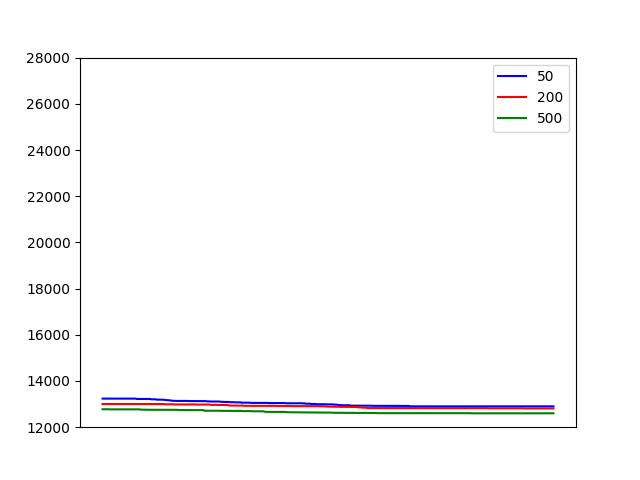
\includegraphics[width=\textwidth]{run_hybrid_lamarckian_20_runs_500_gens.png}
    \caption{500 generations}
  \end{subfigure}
  \hfill
  \begin{subfigure}[b]{0.48\textwidth}
    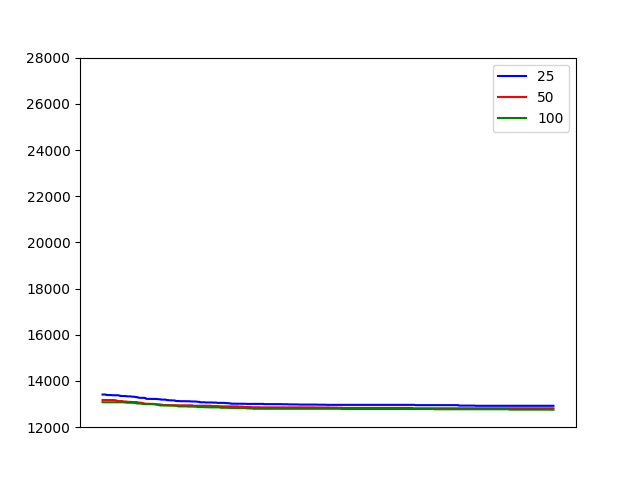
\includegraphics[width=\textwidth]{run_hybrid_lamarckian_20_runs_1000_gens.png}
    \caption{1000 generations}
  \end{subfigure}
  \caption{Plots showing the average best tour in each generaton over 20 runs
    with the Lamarckian version of the hybrid algorithm.}
  \label{fig:hl}
\end{figure}

\end{document}
